\chapter{Scoping}

\section{Primo Project Scoping Meeting}

\subsection{Partecipanti}


\begin{center}
    \begin{tabular}{|l|l|}
        \hline
        \textbf{Ruolo}                   & \textbf{Partecipanti}              \\
        \hline
        Stakeholder                      & Rappresentanti della città di Roma \\
        \hline
        Project Manager                  & Alice Rossi                        \\
        \hline
        Architetti Software              & Giovanni Bianchi, Maria Verdi      \\
        \hline
        Sviluppatori Generici            & Marco Gialli, Laura Neri           \\
        \hline
        Esperti in IoT e Sensoristica    & Luca Azzurri                       \\
        \hline
        Esperti in Sicurezza Informatica & Andrea Blu                         \\
        \hline
        Facilitatore                     & Paolo Rossetti                     \\
        \hline
        Tecnografo                       & Giulia Rossini                     \\
        \hline
    \end{tabular}
\end{center}

\subsection{Agenda}

\begin{enumerate}
    \item \textbf{Introduzione (Facilitatore)}
          \begin{itemize}
              \item Presentazione del team e degli stakeholder presenti.
          \end{itemize}

    \item \textbf{Visione Generale del Progetto (Project Manager)}
          \begin{itemize}
              \item Presentazione del progetto CityTwin e degli obiettivi.
          \end{itemize}

    \item \textbf{Discussione sui Requisiti Utente (Team)}
          \begin{itemize}
              \item Analisi e discussione dei requisiti utente identificati.
          \end{itemize}

    \item \textbf{Definizione dell'Ubiquitous Language (Team)}
          \begin{itemize}
              \item Creazione di un linguaggio comune per il team.
          \end{itemize}

    \item \textbf{Pianificazione dei Prossimi Passi (Team)}
          \begin{itemize}
              \item Discussione sulla struttura del progetto e definizione delle tappe successive.
          \end{itemize}

    \item \textbf{Domande e Risposte (Tutti)}
          \begin{itemize}
              \item Tempo dedicato a domande e chiarimenti.
          \end{itemize}

    \item \textbf{Chiusura del Meeting (Facilitatore)}
          \begin{itemize}
              \item Ringraziamenti e conferma dei prossimi passi.
          \end{itemize}
\end{enumerate}

\subsection{User Stories}

Nel corso del primo incontro di scoping, il team di progetto CityTwin ha identificato e definito le user stories chiave. Questa fase è stata fondamentale per ottenere una comprensione dettagliata delle esigenze degli utilizzatori finali e ha fornito una guida iniziale per lo sviluppo del sistema di digital twin.

\subsubsection{User Story 1: Visualizzazione dello Stato del Sistema tramite GUI}

\textbf{Come} utente interessato al monitoraggio del sistema CityTwin \\
\textbf{Voglio} accedere a una GUI (Control Panel) \\
\textbf{In modo da} visualizzare chiaramente lo stato attuale dei nodi Mainstay e Resource del sistema.

\textbf{Criteri di Accettazione:}
\begin{itemize}
    \item La GUI deve fornire un'interfaccia intuitiva e facile da comprendere.
    \item Lo stato di ciascun nodo (Mainstay e Resource) deve essere chiaramente indicato.
    \item L'utente deve essere in grado di distinguere facilmente i nodi online da quelli offline.
\end{itemize}

\subsubsection{User Story 2: Visualizzazione delle Risorse nella Città tramite GUI}

\textbf{Come} utente interessato alla localizzazione delle risorse nel sistema CityTwin \\
\textbf{Voglio} utilizzare la GUI \\
\textbf{In modo da} visualizzare la posizione delle risorse nella città, con indicazione del nome e dello stato (online/offline).

\textbf{Criteri di Accettazione:}
\begin{itemize}
    \item La mappa nella GUI deve mostrare chiaramente la posizione delle risorse.
    \item Ogni risorsa deve essere contrassegnata con il suo nome e stato di funzionamento.
    \item L'aggiornamento della posizione delle risorse deve essere in tempo reale.
\end{itemize}

\subsubsection{User Story 3: Monitoraggio Storico tramite GUI}

\textbf{Come} utente interessato all'analisi storica dei dati del sistema CityTwin \\
\textbf{Voglio} utilizzare la GUI \\
\textbf{In modo da} visualizzare un grafico che rappresenti il numero di nodi Mainstay e Resource online nel tempo, basato sui dati rilevati dal servizio di persistenza.

\textbf{Criteri di Accettazione:}
\begin{itemize}
    \item La GUI deve presentare un grafico temporale del numero di nodi online nel corso del tempo.
    \item L'asse delle ascisse deve rappresentare il tempo, mentre l'asse delle ordinate deve rappresentare il numero di nodi online.
    \item L'utente deve poter selezionare intervalli temporali specifici per l'analisi.
\end{itemize}

\subsection{Ubiquitous Language}

Durante lo stesso incontro, è stato stabilito un linguaggio comune (Ubiquitous Language) basato sulle specifiche del dominio del progetto CityTwin. Questo linguaggio è stato adottato da tutti i membri del team per garantire una comunicazione chiara e univoca.

\begin{itemize}
    \item \textbf{GUI (Control Panel):} Interfaccia grafica utente che fornisce una visione d'insieme dello stato del sistema CityTwin, consentendo agli utenti di monitorare i nodi Mainstay e Resource.

    \item \textbf{Nodo Mainstay:} Nodo fondamentale all'interno del sistema CityTwin che si occupa di coordinare le informazioni tra i nodi Resource, rilevare malfunzionamenti e salvare dati in modo persistente.

    \item \textbf{Nodo Resource:} Nodo che rappresenta sensori, attuatori o entità complesse all'interno del sistema CityTwin. La composizione di più nodi Resource forma un Digital Twin.

    \item \textbf{Digital Twin:} Rappresentazione digitale di entità fisiche all'interno della città, composta da uno o più nodi Resource.

\end{itemize}

\section{Secondo Project Scoping Meeting}

\subsection{Agenda}

\begin{enumerate}
    \item \textbf{Revisione dei Progressi (Project Manager)}
          \begin{itemize}
              \item Breve riepilogo dei progressi dal primo meeting.
          \end{itemize}

    \item \textbf{Affinamento delle User Stories (Team)}
          \begin{itemize}
              \item Discussione e affinamento delle user stories identificate.
          \end{itemize}

    \item \textbf{Aggiornamento dell'Ubiquitous Language (Team)}
          \begin{itemize}
              \item Revisione e aggiornamento del linguaggio comune.
          \end{itemize}

    \item \textbf{Definizione delle Condition of Satisfaction (Tutti)}

    \item \textbf{Pianificazione delle Attività Future (Team)}
          \begin{itemize}
              \item Discussione sui passi successivi e assegnazione di compiti.
          \end{itemize}

    \item \textbf{Domande e Risposte (Tutti)}
          \begin{itemize}
              \item Tempo dedicato a domande e chiarimenti.
          \end{itemize}

    \item \textbf{Chiusura del Meeting (Facilitatore)}
          \begin{itemize}
              \item Ringraziamenti e conferma dei prossimi passi.
          \end{itemize}
\end{enumerate}

\subsection{User Stories}

In una sessione successiva, il team ha affinato ulteriormente le user stories. Questo passo è stato intrapreso per tenere conto di eventuali nuove informazioni emerse durante lo sviluppo iniziale del progetto, mirando a ottenere una comprensione più approfondita delle esigenze degli utenti.

\subsubsection{User Story 4: Monitoraggio dello Stato del fiume tramite GUI}

\textbf{Come} utente interessato al monitoraggio dello stato dei fiumi \\
\textbf{Voglio} utilizzare la GUI \\
\textbf{In modo da} visualizzare chiaramente lo stato attuale del River Monitor (Safe, Warned, Evacuating).

\textbf{Criteri di Accettazione:}
\begin{itemize}
    \item La GUI deve presentare lo stato corrente del River Monitor in modo evidente.
    \item Lo stato deve essere visivamente distintivo per una rapida interpretazione.
\end{itemize}

\subsubsection{User Story 5: Gestione dello Stato del River Monitor tramite GUI}

\textbf{Come} utente autorizzato alla gestione degli stati del River Monitor \\
\textbf{Voglio} utilizzare la GUI \\
\textbf{In modo da}  poter passare manualmente dallo stato di "Warned" a "Evacuating" e da "Evacuating" a "Safe".

\textbf{Criteri di Accettazione:}
\begin{itemize}
    \item La GUI deve fornire pulsanti chiaramente identificabili per passare tra gli stati.
    \item L'utente autorizzato deve poter effettuare la transizione di stato senza difficoltà.
\end{itemize}

\subsubsection{User Story 6: Aggiunta/Rimozione Nodi Resource in Tempo Reale}

\textbf{Come} amministratore del sistema CityTwin \\
\textbf{Voglio} avere la possibilità di aggiungere o rimuovere nuovi nodi Resource \\
\textbf{In modo da} adattare il sistema alle mutevoli esigenze delle smart city.

\textbf{Criteri di Accettazione:}
\begin{itemize}
    \item L'amministratore deve poter aggiungere nuovi nodi Resource senza interrompere il funzionamento del sistema.
    \item La rimozione di nodi Resource non deve causare problemi di integrità del sistema.
    \item Le modifiche devono essere effettive in tempo reale.
\end{itemize}

\subsection{Conditions of Satisfaction}

Derivate dalle richieste del committente emerse durante il nostro primo incontro, il team ha identificato le seguenti CoS per il progetto:

\begin{enumerate}
    \item \textbf{Vincoli di Budget:} Il completamento del progetto deve avvenire rispettando il budget preventivato per la sua esecuzione.

    \item \textbf{Vincoli di Tempo:} L'implementazione del progetto deve rispettare le tempistiche stabilite, garantendo una consegna puntuale.

    \item \textbf{Soddisfazione del Cliente:} Il prodotto deve non solo soddisfare le esigenze immediate del cliente, ma deve anche costituire una base solida per eventuali sviluppi futuri, assicurando la massima soddisfazione.

    \item \textbf{Rispetto del Piano di Qualità:} È essenziale conformarsi alle convenzioni adottate dalle diverse tecnologie utilizzate e rispettare gli standard concordati in tutte le fasi del progetto, garantendo un livello elevato di qualità.

    \item \textbf{Documentazione Completa dell'Architettura Software:} La documentazione deve essere chiara, completa e facilmente consultabile, pronta a fornire chiarimenti qualora necessario.

    \item \textbf{Modularità:} Il sistema deve essere realizzato in moduli separati, in modo da poter essere facilmente estendibile.

\end{enumerate}


\subsection{Ubiquitous Language}

Durante lo stesso incontro, il linguaggio comune è stato rivisto e aggiornato per riflettere meglio le dinamiche emergenti durante il processo di sviluppo. Questo assicura una comunicazione continua e chiara tra i membri del team.

\begin{itemize}
    \item \textbf{GUI (Control Panel):} Interfaccia grafica utente che fornisce una visione d'insieme dello stato del sistema CityTwin, consentendo agli utenti di monitorare i nodi Mainstay e Resource.

    \item \textbf{GUI (River Monitor):} Interfaccia grafica utente specifica per il monitoraggio dello stato del fiume, consentendo agli utenti di visualizzare informazioni cruciali come lo stato corrente e i livelli dell'acqua.

    \item \textbf{Nodo Mainstay:} Nodo fondamentale all'interno del sistema CityTwin che si occupa di coordinare le informazioni tra i nodi Resource, rilevare malfunzionamenti e salvare dati in modo persistente.

    \item \textbf{Nodo Resource:} Nodo che rappresenta sensori, attuatori o entità complesse all'interno del sistema CityTwin. La composizione di più nodi Resource forma un Digital Twin.

    \item \textbf{Digital Twin:} Rappresentazione digitale di entità fisiche all'interno della città, composta da uno o più nodi Resource.

    \item \textbf{River Monitor:} Parte del sistema CityTwin che si occupa del monitoraggio dello stato dei fiumi, incluso il livello dell'acqua e le transizioni tra gli stati Safe, Warned ed Evacuating.

\end{itemize}

\section{Terzo Project Scoping Meeting}

\subsection{Agenda}

\begin{enumerate}
    \item \textbf{Revisione dei Progressi (Project Manager)}
          \begin{itemize}
              \item Breve riepilogo dei progressi dagli incontri precedenti.
          \end{itemize}

    \item \textbf{Validazione e Convalida delle User Stories (Team)}
          \begin{itemize}
              \item Riveduta e convalida delle user stories alla luce delle informazioni emerse.
          \end{itemize}

    \item \textbf{Consolidamento dell'Ubiquitous Language (Team)}
          \begin{itemize}
              \item Ulteriori raffinamenti e chiarimenti al linguaggio comune.
          \end{itemize}

    \item \textbf{Strutturazione della Requirement Breakdown Structure (Team)}
          \begin{itemize}
              \item Definizione della struttura gerarchica dei requisiti.
          \end{itemize}

    \item \textbf{Definizione del Project Overview Statement}

    \item \textbf{Domande e Risposte (Tutti)}
          \begin{itemize}
              \item Tempo dedicato a domande e chiarimenti.
          \end{itemize}

    \item \textbf{Chiusura del Meeting (Facilitatore)}
          \begin{itemize}
              \item Ringraziamenti e conferma dei prossimi passi.
          \end{itemize}
\end{enumerate}

\subsection{Requisiti}

Sono stati definiti nel dettaglio i requisiti del sistema CityTwin, fornendo una guida chiara per lo sviluppo del progetto. Questa fase è stata fondamentale per ottenere una comprensione approfondita delle funzionalità e delle caratteristiche del sistema.

\subsubsection{Requisiti di Business}
I requisiti aziendali definiscono gli obiettivi di alto livello e la motivazione dietro lo sviluppo del software. Rispondono alla domanda "perché?" e definiscono l'importanza strategica del progetto:
\begin{enumerate}
    \item Obiettivi Strategici: Il progetto "CityTwin" mira a creare una piattaforma di monitoraggio delle smart city per migliorare la gestione e l'ottimizzazione delle risorse urbane.
    \item Aumento dell'Efficienza Urbana: Il sistema mira a migliorare l'efficienza operativa delle città intelligenti attraverso la rappresentazione digitale delle entità e delle interazioni all'interno della città.
\end{enumerate}

\subsubsection{Requisiti Utente}
I requisiti utente si concentrano sull'esperienza dell'utente finale e sulla modalità di interazione con il sistema.
Gli scenari d'uso hanno permesso di definire le azioni principali che gli utenti avrebbero potuto compiere all'interno dell'applicazione.
Per rappresentare in modo efficace questi scenari e facilitare la comunicazione visiva di quello che il sistema offre all'utente, è stato definito un diagramma dei casi d'uso, mostrato in Figura \ref{fig:use-cases-diagram}. Questo diagramma ha contribuito a visualizzare in modo chiaro ed esauriente le attività degli utenti e le interazioni con il sistema.

\begin{enumerate}
    \item L'utente deve avere a disposizione una GUI (Control Panel) con le seguenti funzionalità:
          \begin{enumerate}
              \item Deve mostrare lo stato attuale dei nodi Mainstay e Resource del sistema.
              \item Deve mostrare la posizione delle risorse nella città, indicandone il nome e lo stato (online/offline).
              \item Deve mostrare un grafico che rappresenti il numero di nodi Mainstay e Resource online nel tempo, sulla base dei dati rilevati
                    dal servizio di persistenza.
          \end{enumerate}
    \item L'utente deve avere a disposizione una GUI (River Monitor) con le seguenti funzionalità:
          \begin{enumerate}
              \item Deve mostrare lo stato attuale del River Monitor (Safe, Warned, Evacuating).
              \item Deve mostrare i sensori monitorati con il relativo livello dell'acqua.
              \item Deve mostrare il valore di soglia dell'acqua sopra la quale il River Monitor passa allo stato di "Warned".
              \item Deve mettere a disposizione un pulsante per passare allo stato di "Evacuating" e un pulsante per tornare allo stato di "Safe".
          \end{enumerate}
    \item L'utente deve avere la possibilità di aggiungere o rimuovere nuovi nodi Resource in tempo reale, senza che questo comprometta il funzionamento del sistema. Questa flessibilità consente di adattare il sistema alle mutevoli esigenze delle smart city.
\end{enumerate}
\begin{figure}[H]
    \centering
    \caption{Diagramma dei casi d'uso.}
    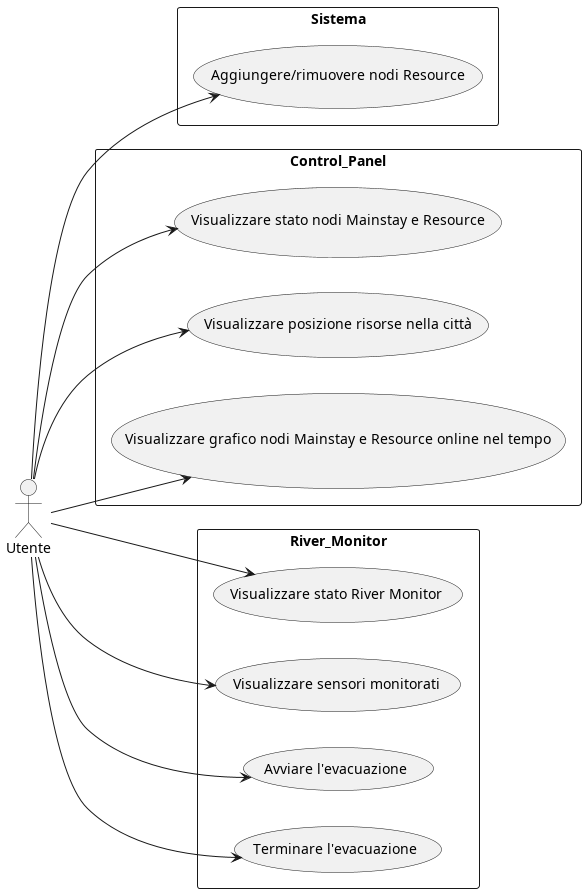
\includegraphics[width=0.8\textwidth]{figures/use-cases-diagram.png}
    \label{fig:use-cases-diagram}
\end{figure}


\subsubsection{Requisiti Funzionali}
I requisiti funzionali delineano le funzioni specifiche del sistema, cioè cosa il sistema deve fare:
\begin{enumerate}
    \item I nodi Mainstay sono la struttura portante dell'intero sistema:
          \begin{enumerate}
              \item Ricevono informazioni dai nodi Resource che modellano sensori.
              \item Comunicano informazioni ai nodi Resource che modellano attuatori.
              \item Rilevano i malfunzionamenti dei nodi Resource.
              \item Rilevano i malfunzionamenti degli altri nodi Mainstay.
              \item Si occupano di salvare le informazioni contattando il servizio di persistenza.
              \item Non devono conoscere a prescindere le tipologie dei nodi Resource.
              \item Devono disporre di una struttura dati distribuita che permetta di memorizzare le informazioni rilevanti:
                    \begin{enumerate}
                        \item La struttura dati deve essere sincronizzata tra i nodi Mainstay.
                        \item La struttura dati deve mantenere la consistenza dei dati nel tempo.
                    \end{enumerate}
          \end{enumerate}
    \item I nodi Resource:
          \begin{enumerate}
              \item Rappresentano astrazioni di:
                    \begin{enumerate}
                        \item Sensori.
                        \item Attuatori.
                        \item Entità più complesse, come stazioni di controllo, che possono anche impiegare interfacce grafiche.
                    \end{enumerate}
              \item Fanno riferimento ad uno dei nodi Mainstay per ottenere o comunicare informazioni.
              \item Possono essere aggiunti o rimossi in tempo reale.
          \end{enumerate}
    \item Deve essere presente un servizio di persistenza dei dati che permetta di salvare in modo persistente:
          \begin{enumerate}
              \item Lo stato dei nodi Mainstay.
              \item Lo stato dei nodi Resource.
          \end{enumerate}
    \item Il malfunzionamento di un nodo non deve compromettere il funzionamento del sistema.
    \item Deve poter essere possibile introdurre nuovi moduli senza dover modificare i componenti esistenti.
    \item Vengono previsti i seguenti moduli per i nodi Resource:
          \begin{enumerate}
              \item Sensore per la rilevazione di piogge acide. Il sensore deve essere in grado di rilevare il valore di pH dell'acqua piovana, compreso tra 0 e 14.
              \item Sensore per l'analisi della qualità dell'aria. Il sensore deve essere in grado di rilevare i seguenti parametri chiave:
                    \begin{enumerate}
                        \item \label{itm:pm10} Concentrazione di PM10 (Particolato inferiore ai 10 micrometri).
                        \item \label{itm:pm25} Concentrazione di PM2,5 (Particolato inferiore ai 2,5 micrometri. Si noti che è un sottoinsieme del PM10).
                        \item \label{itm:NOx} Concentrazione di NOx (Ossidi di azoto).
                    \end{enumerate}
                    Si deve inoltre considerare che si andrà a utilizzare un sensore economico prefabbricato a basso consumo energetico, in grado di comunicare i dati rilevati tramite un protocollo di rete.
              \item Sensore per la rilevazione dell'inquinamento acustico, con le seguenti caratteristiche:
                    \begin{enumerate}
                        \item \label{itm:dB} Le letture devono variare in un intervallo di valori rappresentativi di un ambiente urbano, da 40 a 100 decibel (dB).
                        \item \label{itm:dBDescription} Oltre al valore in decibel, il sensore deve fornire una descrizione corrispondente al livello di rumore.
                    \end{enumerate}
              \item Modulo per la rilevazione del livello dell'acqua di un fiume e possibilità di intervento:
                    \begin{enumerate}
                        \item Sensore per la rilevazione degli allagamenti: il sensore deve periodicamente misurare il livello dell'acqua e comunicare il valore rilevato al nodo Mainstay.
                        \item Pannello di controllo per l'intervento in caso di allagamento, con le seguenti caratteristiche:
                              \begin{enumerate}
                                  \item Soglia di allagamento configurabile.
                                  \item Possibilità di controllare più sensori.
                                  \item Possibilità di assumere tre stati:
                                        \begin{itemize}
                                            \item Safe quando non c'è pericolo.
                                            \item Warned quando il livello dell'acqua supera la soglia di allagamento.
                                            \item Evacuating quando il livello dell'acqua supera la soglia di allagamento e l'utente ha premuto il pulsante di evacuazione.
                                        \end{itemize}
                                  \item Mostrare lo stato attuale del River Monitor.
                                  \item Passaggio in automatico allo stato Warned quando il valore della maggioranza dei sensori supera la soglia di allagamento.
                                  \item Possibilità di intervenire passando in stato Evacuating quando il sistema è Warned.
                                  \item Possibilità di intervenire tornando in stato Safe quando il sistema è Evacuating.
                              \end{enumerate}
                    \end{enumerate}
          \end{enumerate}
\end{enumerate}

\subsubsection{Requisiti Non Funzionali}
I requisiti non funzionali definiscono attributi di qualità, vincoli e proprietà generali del sistema:
\begin{enumerate}
    \item Affidabilità: L'affidabilità e la resilienza sono due aspetti cruciali del sistema "CityTwin". In caso di guasti hardware o malfunzionamenti dei nodi, il sistema deve essere in grado di mantenere la continuità delle operazioni fondamentali. A tale scopo, è prevista l'implementazione di un meccanismo di ridondanza, in cui i dati sono presenti in più istanze di nodi Mainstay.
    \item Performance: Il sistema deve rispondere tempestivamente alle richieste dell'utente (in media entro 1 secondo) e gestire grandi quantità di dati in tempo reale (almeno 30 risorse).
    \item Modularità: Il sistema deve essere realizzato in moduli separati, in modo da poter essere facilmente estendibile.
\end{enumerate}

\subsection{Requirement Breakdown Structure}

Successivamente, il team ha proceduto con riportare i requisiti in un diagramma RBS (Requirement Breakdown Structure), in modo da ottenere una visione d'insieme delle funzionalità e delle caratteristiche del sistema. Questo diagramma è utile soprattutto per il committente del progetto, in quanto fornisce una rappresentazione visiva dei requisiti e delle relazioni tra di essi.

\begin{figure}[H]
    \centering
    \caption{Diagramma dei casi d'uso.}
    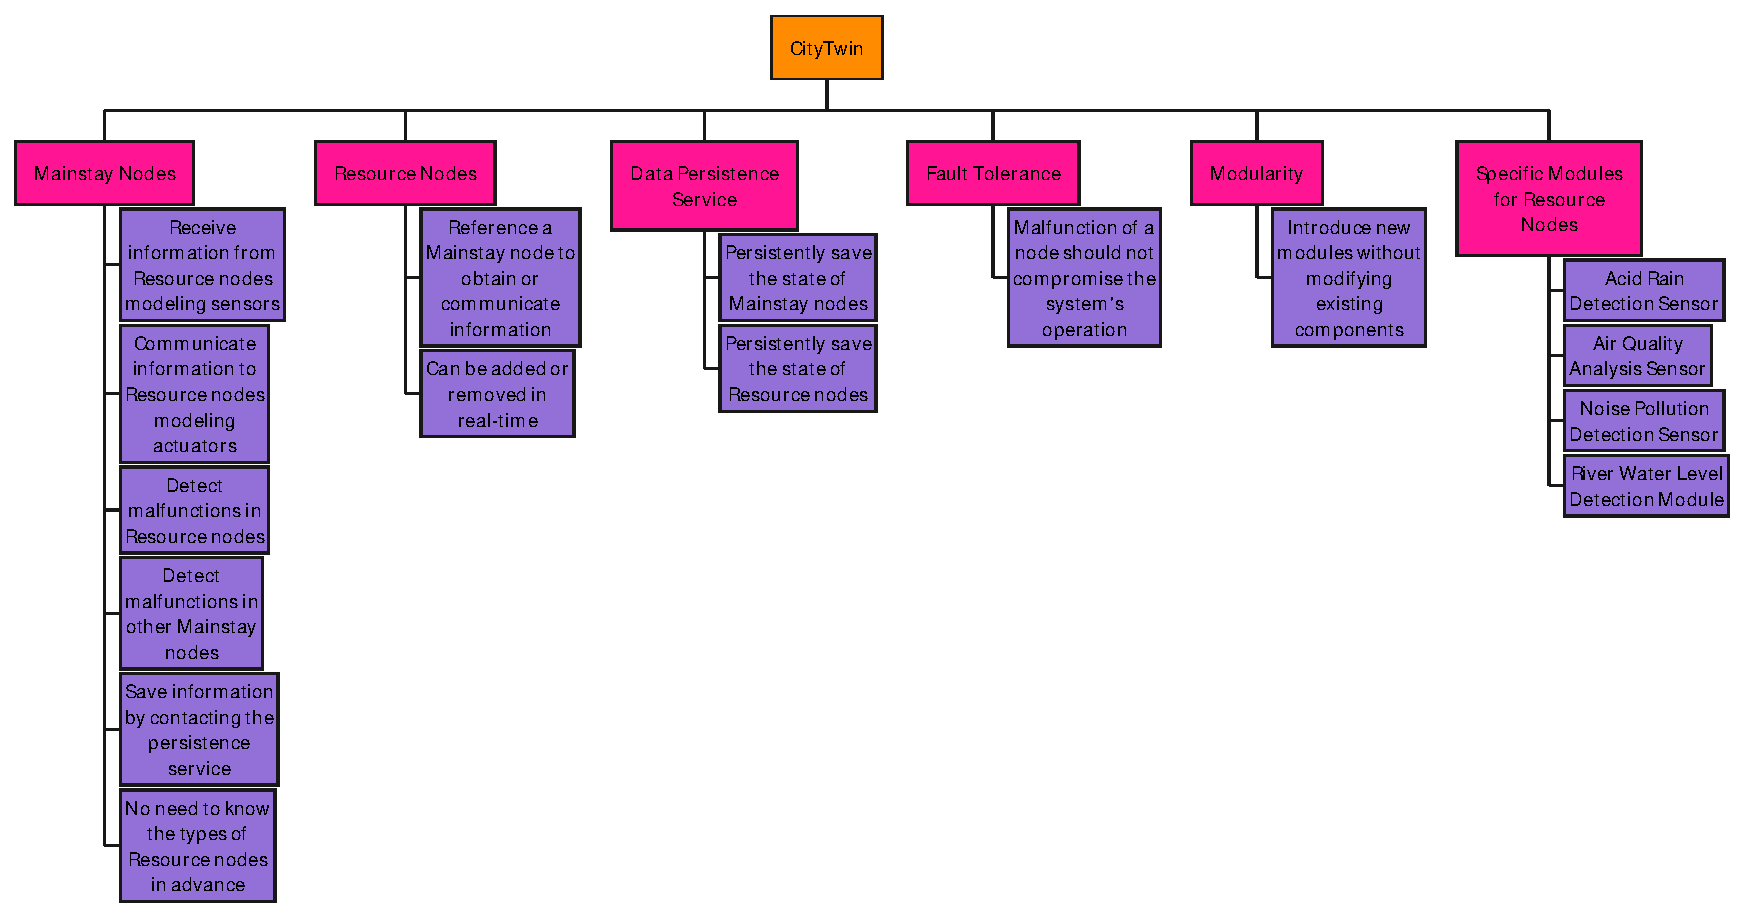
\includegraphics[height=.8\textwidth, angle=90]{figures/RBS.pdf}
    \label{fig:rbs}
\end{figure}

\subsection{Project Overview Statement}

\subsubsection{Problema/Opportunità}

Il progetto CityTwin si propone di affrontare la complessità della gestione urbana attraverso una piattaforma innovativa di monitoraggio delle smart city.

\subsubsection{Goal del Progetto}

L'obiettivo principale di CityTwin è fornire una piattaforma completa e flessibile per il monitoraggio delle smart city, consentendo una gestione efficiente delle risorse urbane e migliorando l'esperienza complessiva degli abitanti.

\subsubsection{Obiettivi del Progetto}

\begin{enumerate}
  \item \textbf{Creazione della Piattaforma:} Sviluppare una piattaforma di monitoraggio, integrando moduli specifici per la gestione avanzata di sensori e attuatori.
  
  \item \textbf{Implementazione di Nodi Mainstay e Resource:} Realizzare nodi Mainstay per la comunicazione efficace e nodi Resource per rappresentare entità urbane, garantendo una gestione dinamica in tempo reale.
  
  \item \textbf{Integrazione di Moduli:} Integrare nuovi moduli, come sensori per la qualità dell'aria e monitoraggio dello stato del fiume, senza compromettere la stabilità del sistema.
\end{enumerate}

\subsubsection{Criteri di Successo}

Il successo del progetto CityTwin sarà valutato in base ai seguenti criteri quantitativi:

\begin{enumerate}
  \item \textbf{Funzionalità Operative:} La piattaforma deve consentire la visualizzazione accurata dello stato della città digitale e il monitoraggio in tempo reale delle risorse.
  
  \item \textbf{Risposta Tempestiva:} Il tempo di risposta del sistema deve rispettare i limiti prestabiliti, garantendo un'esperienza utente efficiente.
  
  \item \textbf{Affidabilità e Ridondanza:} La ridondanza implementata deve mantenere la continuità operativa anche in caso di guasti hardware o malfunzionamenti.
\end{enumerate}

\subsubsection{Assunzioni, Rischi e Ostacoli}

\paragraph{Assunzioni}

\begin{enumerate}
  \item Si assume una collaborazione attiva tra i membri del team e gli stakeholder per garantire una comprensione condivisa degli obiettivi.
  
  \item Si presuppone la disponibilità delle risorse umane e tecnologiche necessarie per lo sviluppo e l'implementazione del progetto.
\end{enumerate}

\paragraph{Rischi e Ostacoli}

\begin{enumerate}
  \item \textbf{Tecnologici:} Rischi legati a nuove tecnologie o tecnologie deprecate.
  
  \item \textbf{Ambienti:} Possibili cambiamenti di personale potrebbero influenzare il progetto.
  
  \item \textbf{Interpersonali:} Gestire le relazioni tra le persone all'interno del team.
  
  \item \textbf{Culturali:} Valutare l'ambito del progetto e la sua convenienza.
  
  \item \textbf{Relazioni Causali:} Assicurare che la soluzione proposta risolva effettivamente il problema identificato.
\end{enumerate}

\subsection{Project Management Life Cycle}

